\pdfbookmark{Общая характеристика работы}{characteristic}             % Закладка pdf
\section*{Общая характеристика работы}

\newcommand{\actuality}{\pdfbookmark[1]{Актуальность}{actuality}\underline{\textbf{\actualityTXT}}}
\newcommand{\progress}{\pdfbookmark[1]{Разработанность темы}{progress}\underline{\textbf{\progressTXT}}}
\newcommand{\aim}{\pdfbookmark[1]{Цели}{aim}\underline{{\textbf\aimTXT}}}
\newcommand{\tasks}{\pdfbookmark[1]{Задачи}{tasks}\underline{\textbf{\tasksTXT}}}
\newcommand{\aimtasks}{\pdfbookmark[1]{Цели и задачи}{aimtasks}\aimtasksTXT}
\newcommand{\novelty}{\pdfbookmark[1]{Научная новизна}{novelty}\underline{\textbf{\noveltyTXT}}}
\newcommand{\influence}{\pdfbookmark[1]{Практическая значимость}{influence}\underline{\textbf{\influenceTXT}}}
\newcommand{\methods}{\pdfbookmark[1]{Методология и методы исследования}{methods}\underline{\textbf{\methodsTXT}}}
\newcommand{\defpositions}{\pdfbookmark[1]{Положения, выносимые на защиту}{defpositions}\underline{\textbf{\defpositionsTXT}}}
\newcommand{\reliability}{\pdfbookmark[1]{Достоверность}{reliability}\underline{\textbf{\reliabilityTXT}}}
\newcommand{\probation}{\pdfbookmark[1]{Апробация}{probation}\underline{\textbf{\probationTXT}}}
\newcommand{\contribution}{\pdfbookmark[1]{Личный вклад}{contribution}\underline{\textbf{\contributionTXT}}}
\newcommand{\publications}{\pdfbookmark[1]{Публикации}{publications}\underline{\textbf{\publicationsTXT}}}

\par	Данная работа посвящена исследованию стабильности динамики тяжелых ионов, а также поляризованных пучков лёгких заряженных частиц в ускорительных и накопительных установках. Представленные результаты направлены на формирование комплексной физической программы исследований, включающей вопросы по разрешению спинового кризиса и изучению электрического дипольного момента элементарных частиц. Также будут разобраны вопросы проектирования современных ускорительных установок.

\par	На сегодняшний день, механизм формирования и эволюции Вселенной остается неразгаданной загадкой. По текущим представлениям, на ранних этапах формирования Вселенной материя находилась в экстремально плотном состоянии, известной как кварк-глюонная плазма \cite{phase_transition_universe}. Подобное состояние материи может наблюдаться в недрах нейтронных звезд \cite{neutron_stars}, а также в результате столкновения тяжелых заряженных частиц. Подобные эксперименты могут осуществляться в рамках коллайдерных исследований и помогут в изучении фазовых переходов и критических явлений в сильновзаимодействующей ядерной материи при экстремальных барионных плотностях \cite{quark_gluon}.

\par	Для достижения статистически значимых результатов любого коллайдерного эксперимента требуется набор достаточного количества статистических данных, что выражается в такой интегральной характеристике как светимость. Обеспечение её высокого уровня является ключевым требованием. Для исследования кварк-глюонной плазмы это требование находится на уровне порядка $10^{27}$~$\text{см}^{-2}\cdot\text{c}^{-1}$ \cite{RHIC_luminosity_heavy}. Такие светимости являются рекордными и для их достижения может потребоваться существенная настройка всех систем ускорителя, что может потребовать большого времени. При ускорении тяжелых ионов высокая зарядность и интенсивность пучка вызывает серьёзные ограничения на параметры сгустка из-за внутрипучкового рассеяния (ВПР) \cite{2016_IBS}. Для преодоления этих проблем, спроектированная структура должна обладать высоким временем ВПР, а также содержать специальные установки стохастического и электронного охлаждения для компенсации эффектов разогрева пучка.

\par	Другой нерешенной проблемой современной физики остается вопрос о распределении спина внутри протона, так называемый "спиновый кризис протона". В 1989 году коллаборацией EMC (European Muon Collaboration) \cite{spin_crisis_1989} было показано, что вклад кварков в спин протона составляет лишь небольшую часть и по современным оценкам находится на уровне около 30$\%$ \cite{quarks_overview_2022}. Исследования этого вопроса проводились при изучении в коллайдерных экспериментах c поляризованными пучками протонов и дейтронов в COSY-ANKE \cite{COSY_ANKE} и SATURNE \cite{SATURNE} при низких энергиях и протонов в RHIC при высоких \cite{RHIC_2014}. 

\par	Для изучения спиновой структуры протонов и дейтронов необходима подготовка и ускорение поляризованных пучков для достижения светимости порядка $10^{32}$ $\text{см}^{-2}\cdot\text{c}^{-1}$ \cite{RHIC_luminosity}. Поляризация пучка является дополнительной степенью свободы, определенные сечения рассеяния приобретают зависимость от поляризации сталкивающихся сгустков. Поскольку соотношение заряда к массе для протона отличается по сравнению с тяжелыми ионами почти в два раза, то максимальная энергия эксперимента кратно увеличивается. В структуре, оптимальной для тяжелоионного эксперимента, подобрано значение критической энергии таким образом, что столкновение происходит до критического значения и никаких проблем по её преодолению не возникает. Критическая энергия является важным параметром ускорительный установки и при проектировании структуры этому вопросу уделяется особое внимание. Таким образом, для протонов прохождение критической энергии становится важным параметром, ограничивающем параметры сгустка, и требует принятия дополнительных мер для её преодоления.

\par	При ускорении протонного пучка относительно длительное нахождение вблизи критической энергии или её пересечение существенно влияет на динамику пучка и его стабильность. Нарушается адиабатичность продольного движения, существенными становятся нелинейные эффекты, затухание Ландау оказывается неспособно подавить возникающие возмущения, а наличие пространственного заряда и других импедансов оказывает влияние на развитие продольной микроволновой неустойчивости, нестабильности отрицательной массы и поперечной голова-хвост (head-tail) \cite{ng, lee}. В случае малых интенсивностей критическая энергия не оказывает значительного влияния на параметры сгустка. Проблема прохождения критической энергии является характерной для интенсивных сгустков с количеством частиц порядка $10^{10}-10^{12}$. Высокая интенсивность в коллайдерных экспериментах, обусловлена требованиями по достижению высокого значения светимости. Однако, любое увеличение эмиттанса пучка приводит к снижению конечной светимости эксперимента. Влияние всех приведенных эффектов, ограничено временем нахождения вблизи критической энергией, в этой связи используются методы быстрого пересечения или поднятия критической энергии.

\par	Известная проблема физики состоит в объяснении барионной асимметрии, то есть наблюдаемым преобладанием материи над антиматерией. До сих пор, существующие физические законы не способны полностью объяснить такой дисбаланс. В работе 1967 год А. Д. Сахаровым были сформулированы общие необходимые условия для наличия барионной асимметрии: 1) Нарушение закона сохранения барионного заряда; 2) Нарушение C- и CP-симметрии; 3) Нарушение на ранних этапах формирования Вселенной термодинамического равновесия \cite{sakharov}. Согласно второму условию, "\textit{Возникновение С-асимметрии по нашей гипотезе является следствием нарушения СР-инвариантности при нестационарных процессах расширения горячей Вселенной на сверхплотной стадии, которое проявляется в эффекте различия парциальных вероятностей зарядово-сопряженных реакций}".  Ранее в 1958 году С. Окубо теоретически показал такой эффект при рассмотрении распада сигма гиперона $\Sigma^{+}$ и его античастицы $\bar{\Sigma}^{+}$. Позднее в 1964 году Д. Кронин и В. Фитч экспериментально обнаружили нарушение CP-инвариантности слабого взаимодействия в процессах распада нейтральных каонов $K_{2}^{0}$ на два пиона $\pi^{+}, \pi^{-}$ \cite{CP}, за что в 1980 году были удостоены нобелевской премии по физике. 

\par	В современной Стандартной модели частиц P-\cite{P-violation} и CP-симметрии нарушаются. Источником CP-нарушения является наличие комплексной фазы в матрице смешивания кварков Кабиббо-Кабаяси-Маскава для слабых взаимодействий \cite{CKM} и коэффициента $\theta_{\text{QCD}}$ в лагранжиане квантовой хромодинамики \cite{CPstrong}, однако не обнаружено CP-нарушений в сильных взаимодействиях. Согласно CPT-теореме, CP-инвариантность эквивалентна T-инвариантности. Источником такого нарушения может являться ненулевой электрический дипольный момент (ЭДМ) элементарных частиц, фундаментальное свойство материи и обусловленное неоднородностью распределения заряда внутри частицы. Поскольку ЭДМ представляется полярным вектором, а не псевдовектором, то для него нарушается как P-, так и T-инвариантность, что показано на рис. \ref{fig:4edmpt}.  Величина ЭДМ в Стандартной Модели слишком мала для экспериментального детектирования и находится на уровне $\abs{d_{n}}< 10^{-30}-10^{-32}$ $e\cdot \text{см}$ для нейтрона \cite{EMD_overview}. Возможность его существования была сформулирована в заметке 1950 Перселл и Рэмси \cite{EDM}, однако ненулевое ЭДМ пока точно не обнаружено. Другие теоретические модели, такие как Суперсимметричные (SUSY), также предсказывают наличие ЭДМ, но на уровне $\abs{d_{n}}< 10^{-27}-10^{-29}$ $e\cdot \text{см}$ для нейтрона, которые оставляют существенную надежду на экспериментальное обнаружение. Стоит отметить, что и таких точностей пока достигнуто не было, а сделаны только существенные ограничения для нейтрального нейтрона, впервые появившиеся в работе Н. Рамси и его коллег $\abs{d_{n}}< 5\times10^{-20}$ $e\cdot \text{см}$ ($90\%$ C.L.) \cite{NeutronEDM}, текущее ограничение находится на уровне $\abs{d_{n}}< 1.8\times 10^{-26}$ $e\cdot \text{см}$ ($90\%$ C.L.), что получено в работе nEDM \cite{neutron_EDM_current}.

\begin{figure}
	\centering
	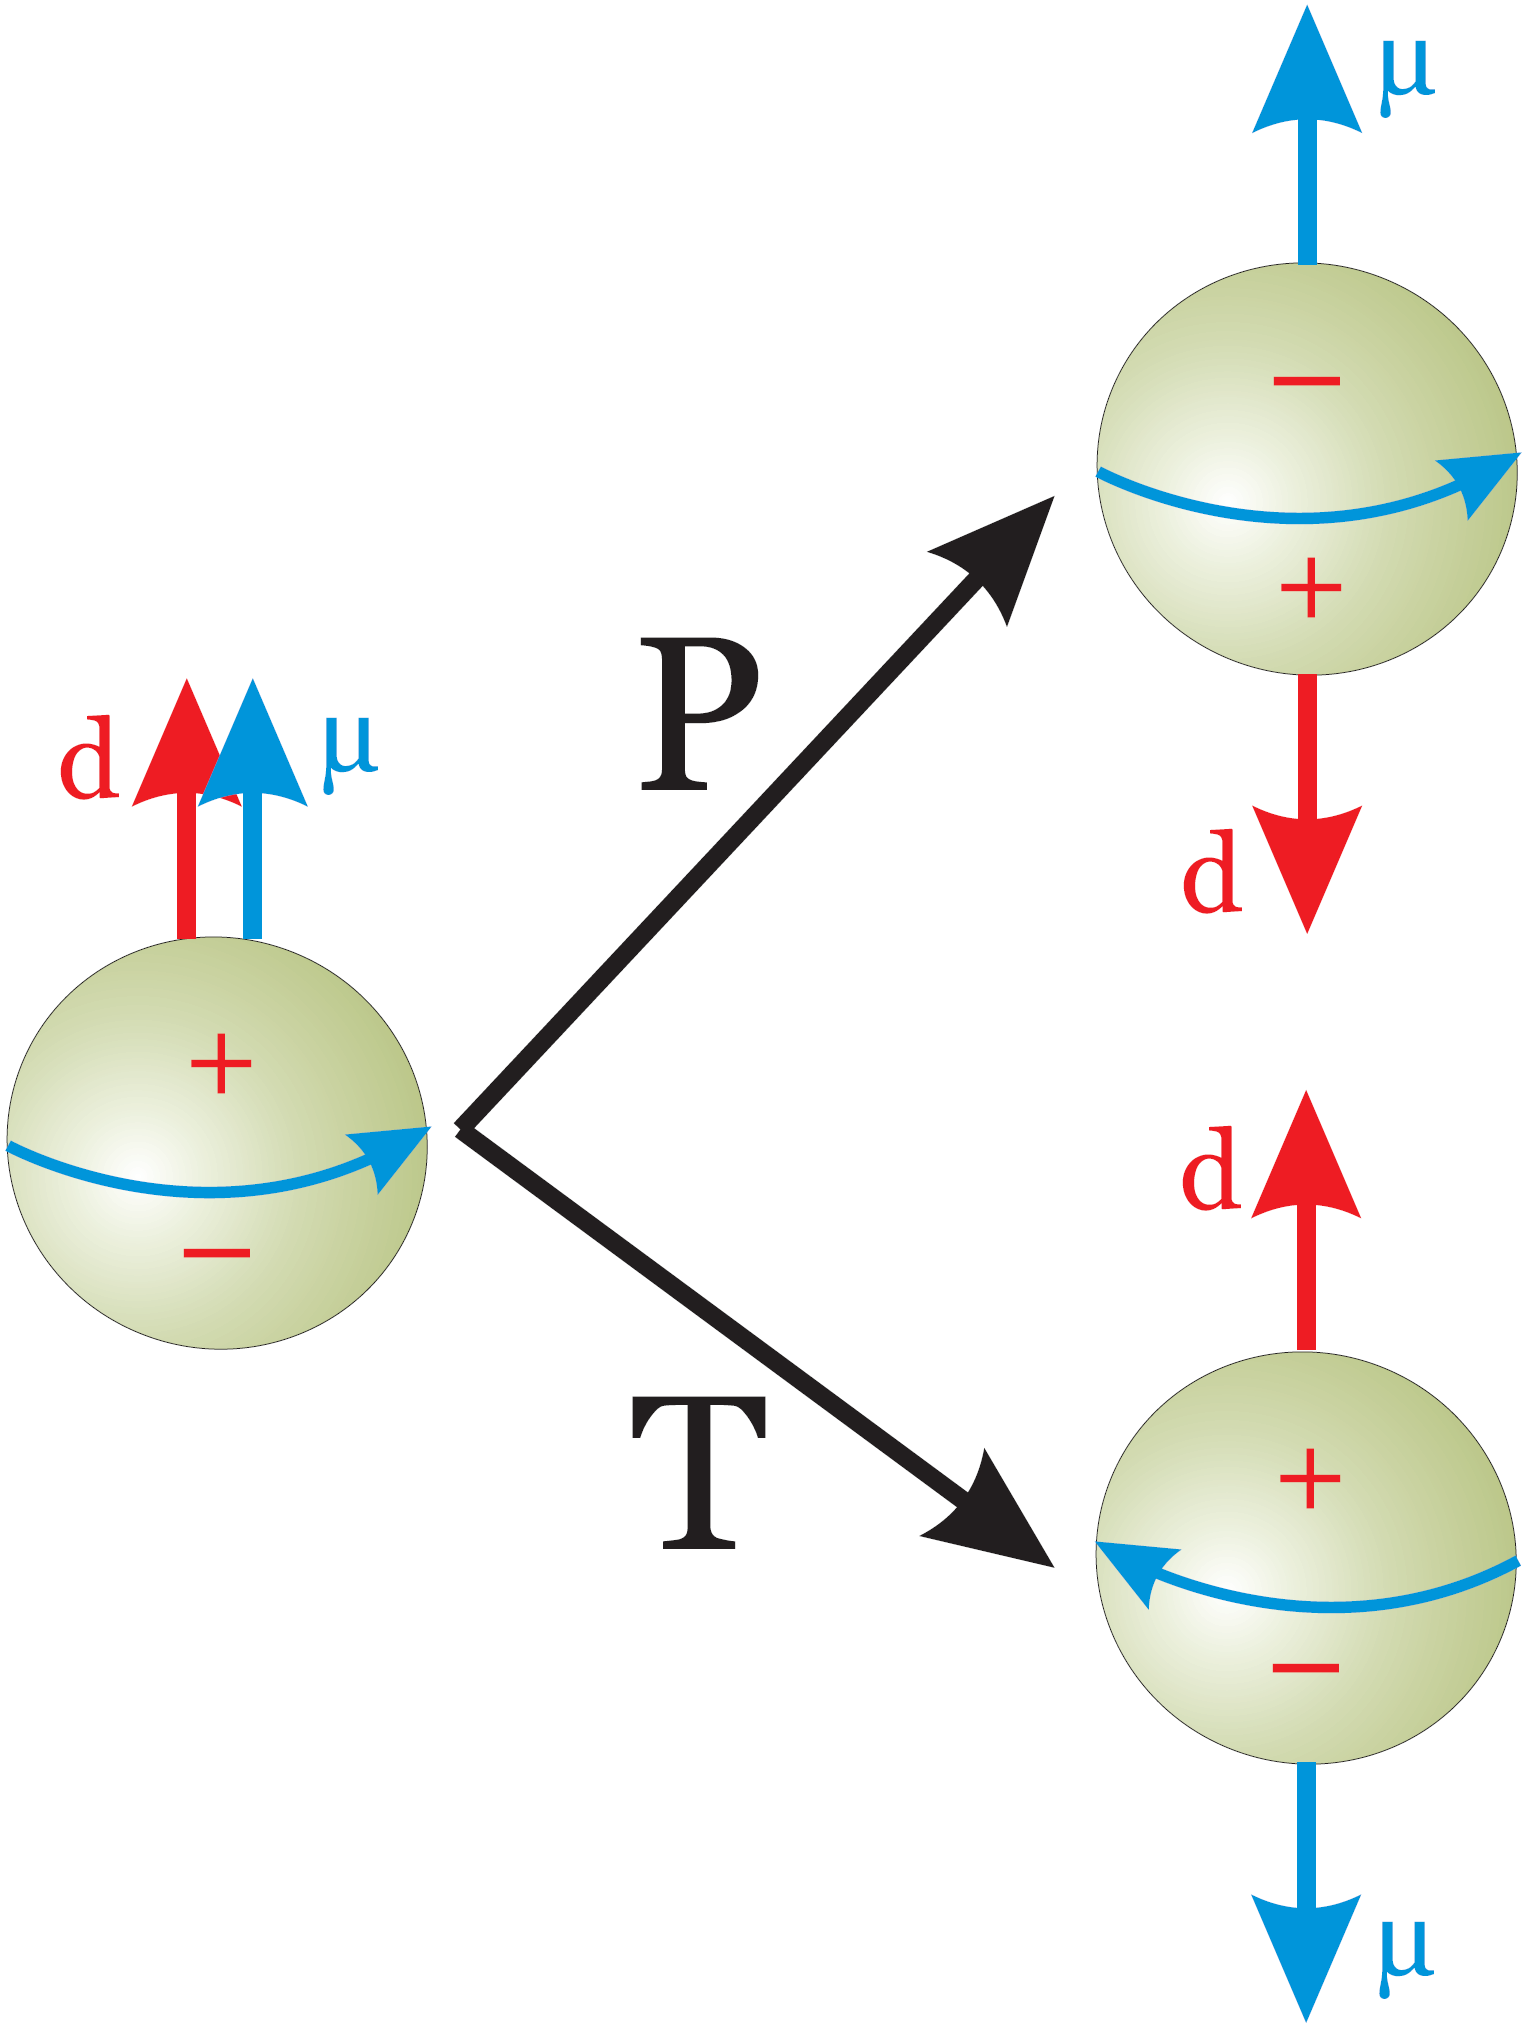
\includegraphics[width=0.4\linewidth]{images/4_EDM_P_T}
	\caption{Схематическое изображение нарушение P- и Т-симметрии ненулевым электрическим дипольным моментом.}
	\label{fig:4edmpt}
\end{figure}

\par	Исследование ЭДМ осуществляется согласно уравнению Т-БМТ по его влиянию на поведение поляризации в электромагнитных полях. В случае ЭДМ нейтрона, а также нейтральных атомов их положение сохраняется при действии внешних магнитных и электрических полей. В случае заряженных частиц происходит движение согласно силе Лоренца, что и приводит к необходимости применения ускорительных установок, позволяющих длительное накопление пучка с заданными параметрами и выступающих в роли накопительного кольца. Наиболее интересным и перспективным направлением выглядит изучение ЭДМ протона и дейтрона. Для этого требуется создание когерентных пучков. Тогда сохраняется поляризация вдоль конкретной оси, а также спины частиц прецессируют с одинаковой частотой. Для накопления малой величины ЭДМ необходимо долгое удержание пучка с последующим анализом рассеяния на мишени поляриметра. При этом влияние магнитного дипольного момента (МДМ) должно быть подавлено. Такая техника впервые была предложена в БНЛ (Брукхейвенская Национальная Лаборатория) и имеет название 'замороженный' спин \cite{Farley:edm}. Позднее, была предложена концепция 'квази-замороженного' спина \cite{QFS}, в которой происходит пространственное разделение полей и интегральное подавление МДМ-компоненты за полный оборот по кольцу.

\par	Ещё одним перспективным направлением исследований в рамках программы спиновой физики является исследование аксиона. В этом случае резонансным методом между частотой спиновой прецессии и частотой осциллирующего скалярного аксионового поля может быть получена масса аксиона или установлены соответствующие ограничения. Для этого ускоритель будет использован в роли зондирующей антенны по частоте прецессии спина \cite{Axion_Nikolaev}.

\par	Приведённые вопросы фундаментальной физики подлежат детальному рассмотрению и могут быть исследованы с использованием ускорительных установок, предназначенных для проведения разнообразных экспериментов. Эти установки позволяют достигать высоких энергий частиц, а также предельных точностей измерений. Такая практика применяется в крупных мировых ядерных центрах: CERN \cite{lhc:heavy_ions}, BNL \cite{rhic:design}, J-PARC \cite{j-park}. Последовательные программы экспериментов расписаны на годы и десятилетия вперед. В первую очередь такие установки служат для фундаментальных исследований, но также поддерживают широкий спектр прикладных задач в таких областях, как медицина, материаловедение и информационные технологии. Кроме того, ускорительные комплексы способствуют развитию необходимых технологий, что укрепляет научно-техническую базу и формирует долгосрочные положительные эффекты. Они также служат важной образовательной платформой, формируя программы для обучения молодых специалистов и предоставляют уникальные возможности для их профессионального роста. 

\par	Ускорительный комплекс NICA (Nuclotron-based Ion Collider fAсility) является современным передовым центром, который оборудован передовой материально-технической базой, отвечающей мировым тенденциям и формируется на базе ОИЯИ в городе Дубна, Россия \cite{nuclotron24}. Основной установкой комплекса является коллайдер, в котором предусмотрены два места встречи пучков, где расположены два детектора: MPD (Multi-Purpose Detector) и SPD (Spin Physics Detector) \cite{Ladygin:SPD}. Каждый из этих детекторов предназначен для различных экспериментов. MPD-детектор будет использован для исследования кварк-глюонной плазмы, возникающей в результате столкновения тяжёлых ионов \cite{MPD, Tech_NICA}. SPD-детектор направлен на изучение поведения сталкивающихся поляризованных пучков протонов и дейтронов. Кинематическая область, охватываемая SPD, уникальна и никогда не использовалась целенаправленно при поляризованных адронных столкновениях. Кроме того, уникальной возможностью станет изучение поляризованных дейтронов. Таким образом, структура коллайдера должна поддерживать ускорение как тяжёлых ионов, так и лёгких частиц. При этом требования к удержанию пучков для различных типов частиц существенно отличаются.

~\\
\par {\actuality} Исследования направлены на формирование полноценной физической программы по изучению динамики поляризованных пучков в комплексе Nuclotron-NICA. Применение изложенных в работе подходов возможно и на других похожих установках без потери общности.
~\\
\par {\aim} данной диссертации является изучение особенностей динамики лёгких поляризованных пучков для проведения коллайдерных экспериментов в дуальной структуре, а также исследования электрического дипольного момента с использованием квази-замороженной концепции.
Для достижения поставленной цели необходимо было 
решить следующие {\tasks}:
\begin{enumerate}[beginpenalty=10000] % https://tex.stackexchange.com/a/476052/104425
	\item	Определение требований к дуальной структуре для тяжелых ионов;
	\item	Регулирование критической энергии для поляризованных частиц методом резонансной модуляции дисперсионной функции;
	\item	Проведение численного моделирования динамики пучка легких частиц с учетом высших порядков коэффициента уплотнения орбиты в высокочастотых резонаторах гармонического и барьерного типа;
	\item 	Поведение динамической апертуры с учетом высших порядков при прохождении пучка через критическую энергию с скомпенсированной хроматичностью;
	\item 	Особенности поведения поляризации пучка при совершении процедуры скачка критической энергии;
	\item 	Изучение концепции «квази-замороженного» спина с целью создания установки для исследования ЭДМ дейтрона и протона;
	\item	Исследование спин-орбитального движения поляризованного пучка в магнитном кольце с фильтрами Вина;
\end{enumerate}
\begin{comment}
\begin{enumerate}[beginpenalty=10000] % https://tex.stackexchange.com/a/476052/104425
  \item Расчёт времени внутрипучкового рассеяния для тяжелых ионов;
  \item Оценка влияния методов с стохастического охлаждения пучка на время жизни;
  \item Моделирование магнитооптики с модулированной дисперсионной функцией;
  \item Проведение численного моделирования продольной динамики частиц с учетом высших порядков коэффициента уплотнения орбиты в высокочастотых резонаторах гармонического и барьерного типа;
  \item Обеспечение стабильности пучка с точки зрения динамической апертуры при процедуре скачка критической энергии, подавление хроматичности, компенсация нелинейных эффектов;
  \item Сохранение поляризации пучка при совершении процедуры скачка критической энергии;
  \item Изучение концепции «квази-замороженного» спина с целью создания установки для исследования ЭДМ дейтрона и протона;
  \item Спин-орбитальное моделирование в магнитном кольце с дополнительными элементами со скрещенными магнитными и электрическими полями;
\end{enumerate}
\end{comment}
~\\
\par {\novelty}
\begin{enumerate}[beginpenalty=10000] % https://tex.stackexchange.com/a/476052/104425
	\item	Впервые предложена дуальная структура для тяжелых ионов и легких частиц для коллайдера NICA;
	\item 	Впервые предложены методы подавления дисперсии поворотной аркой в резонансной магнитооптической структуре с отсутствующими магнитами;
	\item 	Впервые исследован метод скачка критической энергии с использованием барьерного ускоряющего потенциала с учётом ограничений по продольной микроволновой неустойчивости;
	\item	Были проведены исследования продольной динамики с учётом высших порядков разложения по импульсу, а также влиянием импеданса. На их базе сформулированы ограничения на величину и темп скачка критической энергии;
	\item	Были разработаны 8- и 16-периодичная квази-замороженная структура Nuclotron для выделения ЭДМ сигнала легких ядер;
	\item	Была разработана структура коллайдера NICA с обводными каналами, неориентированная изначально на эксперименты по поиску ЭДМ дейтрона методом квази-замороженного спина;
\end{enumerate}
\begin{comment}
	\item	Исследованы закономерности динамики многозарядных тяжёлых ионов и лёгких поляризованных частиц в дуальной магнитооптической структуре с учётом различий во внутрипучковом рассеянии и влияния критической энергии на устойчивость пучка;
 	\item 	Предложен метод резонансной модуляции дисперсионной функции с применением дополнительного семейства квадрупольных линз, что позволило повысить критическую энергию и стабильность пучка в режиме ускорения лёгких частиц;
 	\item	Приведены способы подавления дисперсии на краях поворотных арок в отсутствии регулярности, а также способы подавления нелинейных эффектов;
 	\item 	Выполнено численное моделирование прохождения критической энергии с учётом высших порядков зависимости от импульсного разброса, а также влияния импедансов, что позволило количественно оценить влияние данных факторов на сохранение пучка;
 	\item	Исследована продольная динамика поляризованного пучка при нахождении вблизи и прохождении критической энергии методом скачка в гармоническом и барьерном ВЧ, что позволило количественно оценить стабильность пучка в различных режимах ускорения;
 	\item	Предложено применение метода фильтров Вина для сохранения направления поляризации в пучках, что расширяет возможности по исследованию электрического дипольного момента и аксионоподобных частиц;
 	\item	Рассмотрены вариации изучения ЭДМ дейтрона и протона в много-периодичных структурах с использованием электростатических дефлекторов или фильтров Вина;
\end{comment}
~\\
\par {\influence}:
\par Исследование динамики пучка вблизи критической энергии показывает необходимость её преодоления, а также  способствует определению оптимальных параметров скачка критической энергии. Определено существенное влияние критической энергии на динамику поляризованного протонного пучка.

\par В качестве решения проблем с тяжелыми и легкими частицами разработана дуальная структура. Дуальность структуры указывает на возможность её эффективного решения обоих эффектов и использования сразу для двух фундаментально значимых исследований: для изучения кварк-глюонной плазмы в коллайдерных экспериментах с тяжелыми ионами и для исследования легких поляризованных пучков в симметричных и асимметричных коллайдерных столкновениях.

\par Расширена применимость метода «резонансных структур» для случая отсутствия периодичности дисперсионной функции на арках.

\par В части поляризованных частиц адаптирован метод “квази-замороженного спина” для коллайдера NICA, продемонстрировавший возможность проведения исследований по электрическому дипольному моменту без значительных изменений структуры ускорителя. Разработана магнитооптическая структура обводных каналов bypass, позволяющая обойти точки встречи для обоих детекторов с расположенными на них прямыми фильтрами Вина. Данная схема позволяет реализовать концепцию "квази-замороженного спина" для исследования электрического дипольного момента дейтрона. 

\par Методы разработанные для кольца NICA могут быть использованы и для Nuclotron с сохранением функций бустера для поляризованного пучка в коллайдер. Это также позволит проведение независимых экспериментов по исследованию ЭДМ и поиску аксиона. Такие исследования является отдельной частью программы спиновой физики, которая формируется на уста­новке NICA-Nuclotron.


% {\progress}
% Этот раздел должен быть отдельным структурным элементом по
% ГОСТ, но он, как правило, включается в описание актуальности
% темы. Нужен он отдельным структурынм элемементом или нет ---
% смотрите другие диссертации вашего совета, скорее всего не нужен.
~\\
\par {\methods} Основными методами исследования являются математическое и компьютерное моделирование, численный эксперимент. Для исследования были использованы программы для расчёта поперечной динамики: MAD-X \cite{madx}, OPTIM \cite{optim}, BMAD \cite{bmad}, продольной динамики: BLonD \cite{blond}; спин-орбитальной динамики: COSY Infinity \cite{cosy}.
~\\
%второй вариант
\begin{comment}
\par {\defpositions}
\begin{enumerate}[beginpenalty=10000] % https://tex.stackexchange.com/a/476052/104425
  \item 	Принципы построения дуальной магнитооптической структуры с оптимизированным временем жизни пучка в регулярной структуре для многозарядных тяжелых ионов и варьированной критической энергией в резонансной структуре для легких ядер; \cite{Kolokolchikov:2025_dual}, \cite{Syresin:2021_polar}
  \item	Результаты, полученные в эксперименте на У-70 и в методе численного моделирования динамики продольного движения вблизи критической энергии с учётом влияния высших порядков зависимости от разброса по импульсу и с учетом импеданса; \cite{Kolokolchikov:2025_U70}, \cite{Kolokolchikov:2025_jump}
  \item	Результаты исследования продольной динамики поляризованного пучка для процедуры скачка критической энергии в гармоническом и барьерном ВЧ, оценка влияния продольной микроволновой неустойчивости; \cite{Kolokolchikov:2024_bb_rupac}, \cite{Kolokolchikov:2023_bb_IPAC}, \cite{Kolokolchikov:2024_bb_dspin}
  \item	Метод подавления дисперсии и влияния нелинейных эффектов, из-за нарушения периодичности за счет введения missing magnet на краях поворотных арок, для создания резонансной магнитооптической структуры; \cite{Kolokolchikov:2021trans}, \cite{Kolokolchikov:2023_pecular}
  \item	Модернизированная структура с квази-замороженным спином для исследования ЭДМ дейтронов и протонов и возможностью совместного использования Нуклотрона в качестве бустера поляризованных частиц для коллайдера; \cite{Senichev:2023_QFS}, \cite{Senichev:2023_nuclotron}, \cite{Kolokolchikov:2025_nuclotron}
  \item	Метод обводных каналов bypass для независимого исследования ЭДМ в кольце коллайдера;\cite{Kolokolchikov:2023_bypass}, \cite{Kolokolchikov:2023_bypass_IPAC}, \cite{Senichev:2024_nica_edm}, \cite{Kolokolchikov:2023_sc}, \cite{Kolokolchikov:2023_sc_IPAC}
\end{enumerate}
\end{comment}

%третий вариант
\begin{comment}
\par {\defpositions}
\begin{enumerate}[beginpenalty=10000] % https://tex.stackexchange.com/a/476052/104425
  \item 	Изучение внутрипучкового рассеяния и стохастического охлаждения для оптимизации времени жизни пучка в регулярной структуре для многозарядных тяжелых ионов и варьированной критической энергией в резонансной структуре для легких ядер с целью реализации дуальности ускорительной установки; \cite{Kolokolchikov:2025_dual}, \cite{Syresin:2021_polar}
  \item	Результаты, полученные в эксперименте на У-70 и в методе численного моделирования динамики продольного движения вблизи критической энергии с учётом влияния высших порядков зависимости от разброса по импульсу и с учетом импеданса; \cite{Kolokolchikov:2025_U70}, \cite{Kolokolchikov:2025_jump}
  \item	Результаты исследования продольной динамики поляризованного пучка для процедуры скачка критической энергии в гармоническом и барьерном ВЧ, оценка влияния продольной микроволновой неустойчивости; \cite{Kolokolchikov:2024_bb_rupac}, \cite{Kolokolchikov:2023_bb_IPAC}, \cite{Kolokolchikov:2024_bb_dspin}
  \item	Метод подавления дисперсии и влияния нелинейных эффектов в резонансной магнитооптической структуре из-за нарушения периодичности по дисперсии за счет missing magnet на краях поворотных арок; \cite{Kolokolchikov:2021trans}, \cite{Kolokolchikov:2023_pecular}
  \item	Модернизированная структура с квази-замороженным спином для исследования ЭДМ дейтронов и протонов и возможностью совместного использования Нуклотрона в качестве бустера поляризованных частиц для коллайдера; \cite{Senichev:2023_QFS}, \cite{Senichev:2023_nuclotron}, \cite{Kolokolchikov:2025_nuclotron}
  \item	Метод введения обводных каналов в кольцо синхротрона для создания независимой установки с возможностью проведения прецизионных экспериментов, в том числе изучения ЭДМ элементарных частиц;\cite{Kolokolchikov:2023_bypass}, \cite{Kolokolchikov:2023_bypass_IPAC}, \cite{Senichev:2024_nica_edm}, \cite{Kolokolchikov:2023_sc}, \cite{Kolokolchikov:2023_sc_IPAC}
\end{enumerate}
\end{comment}

\begin{comment}
\par {\defpositions}
\begin{enumerate}[beginpenalty=10000] % https://tex.stackexchange.com/a/476052/104425
  \item 	Основные свойства дуальной магнитооптической структуры для легких ядер и тяжелых частиц с учетом различия внутрипучкового рассеяния. Время жизни пучка в дуальной структуре с учетом вариации коэффициента проскальзывания в разных арках; \cite{Kolokolchikov:2025_dual}, \cite{Syresin:2021_polar}
  \item	Учет влияния высших порядков разброса по импульсам и моделей продольных импедансов в численном моделировании движения в окрестности критической энергии и сравнение с экспериментальными результатами, полученными на У-70; \cite{Kolokolchikov:2025_U70}, \cite{Kolokolchikov:2025_jump}
  \item	Результаты математического моделирования процесса прохождения ансамбля частиц через критическую энергию с различной скоростью и при различной форме ускоряющего потенциала с учетом ограничений по продольной микроволновой неустойчивости; \cite{Kolokolchikov:2024_bb_rupac}, \cite{Kolokolchikov:2023_bb_IPAC}, \cite{Kolokolchikov:2024_bb_dspin}
  \item	Резонансная модуляция дисперсионной функции, как метод вариации критической энергии. Результаты оптимизации дисперсионной функции при наличии отсутствующих магнитов (missing magnets); \cite{Kolokolchikov:2021trans}, \cite{Kolokolchikov:2023_pecular}
  \item	Особенности поляризованных пучков, используемых для исследования электрического дипольного момента в структурах с квази-замороженным спином на примере модернизированной структуры Нуклотрона; \cite{Senichev:2023_QFS}, \cite{Senichev:2023_nuclotron}, \cite{Kolokolchikov:2025_nuclotron}
  \item	Метод фильтров Вина для сохранении направления поляризации  на основе введения обводных каналов в структуре с квази-замороженным спином для выделения ЭДМ сигнала в поляризованном пучке;\cite{Kolokolchikov:2023_bypass}, \cite{Kolokolchikov:2023_bypass_IPAC}, \cite{Senichev:2024_nica_edm}, \cite{Kolokolchikov:2023_sc}, \cite{Kolokolchikov:2023_sc_IPAC}
\end{enumerate}
\end{comment}

\par {\defpositions}
\begin{enumerate}[beginpenalty=10000] % https://tex.stackexchange.com/a/476052/104425
	\item 	Предложена реализация дуальной структуры для комплекса NICA-Nuclotron, оптимальная для тяжелых частиц с точки зрения внутрипучкового рассеяния и легких частиц с поднятой критической энергией выше энергии эксперимента; \cite{Kolokolchikov:2025_dual, Syresin:2021_polar}
	\item	Реализован метод вариации критической энергии для магнитооптики коллайдера NICA с отсутствующими магнитами при подавлении дисперсионной функции двумя семействами квадруполей и двумя крайними ячейками поворотной арки; \cite{Kolokolchikov:2021trans, Kolokolchikov:2023_pecular}
	\item	Представлены результаты численного моделирования продольной динамики с учетом влияния высших порядков разброса по импульсам и моделей продольных импедансов в окрестности критической энергии и сравнение с экспериментальными результатами, полученными на У-70; \cite{Kolokolchikov:2025_U70, Kolokolchikov:2025_jump}
	\item 	Проведен анализ использования гармонического ВЧ при процедуре скачка в коллайдере NICA. Для барьерного ВЧ представлены данные моделирования продольной динамики, а также предложено сокращение длины между барьерами из-за продольной микроволновой неустойчивости; \cite{Kolokolchikov:2024_bb_rupac, Kolokolchikov:2023_bb_IPAC, Kolokolchikov:2024_bb_dspin}
	\item	Предложены модернизированные квази-замороженные 8/16-периодичные структуры Nuclotron для исследования электрического дипольного момента легких ядер, с сохранением функции бустера. \cite{Senichev:2023_QFS, Senichev:2023_nuclotron, Kolokolchikov:2025_nuclotron}
	\item	Применен метод фильтров Вина для сохранении направления поляризации на основе введения обводных каналов в структуре коллайдера NICA с квази-замороженным спином для выделения ЭДМ сигнала в поляризованном пучке дейтронов;\cite{Kolokolchikov:2023_bypass, Kolokolchikov:2023_bypass_IPAC, Senichev:2024_nica_edm, Kolokolchikov:2023_sc, Kolokolchikov:2023_sc_IPAC}
\end{enumerate}

~\\
\par {\reliability} полученных результатов подтверждается согласованием аналитических вычислений с результатами численных экспериментов. Результаты находятся в соответствии с результатами, полученными другими авторами.
~\\
\par {\probation}
Основные результаты работы были представлены докладывались~на российских и международных конференциях, а также рабочих встречах: 
\begin{itemize}
\item Workshop “Polarized beam in NICA” в 2022 г.;
\item Молодежная конференция по теоретической и экспериментальной физике МКТЭФ-2020. Москва, Россия;
\item 63, 65, 66-ая Всероссийская научная конференция МФТИ в 2020, 2023, 2024 гг. г. Долгопрудный,
Россия;
\item XXVII и XXVIII Всероссийская конференции по ускорителям заряженных частиц RuPAC'21, RuPAC'23. Алушта; Новосибирск, Россия.
\item VII, VIII, IX и X Международная конференция Лазерные и Плазменные технологии ЛаПлаз'21, ЛаПлаз'22, ЛаПлаз'23, ЛаПлаз'24, ЛаПлас'25. Москва, Россия;
\item XIII, XIV, XVI международная конференция по ускорителям заряженных частиц IPAC'22 IPAC'23, IPAC'25. Бангкок, Тайланд; Венеция, Италия; Тайпей, Тайвань;
\item XIX Международная конференции по спиновой физике высоких энергий DSPIN'23. Дубна, Россия;
\item XI-я Международная конференция по ядерной физике в накопительных кольцах STORI’24. Хуэйчжоу, провинция Гуандун, Китай;
\end{itemize}
~\\
\par {\contribution} Все результаты, выносимые на защиту, получены автором лично, либо при его непосредственном участии. Содержание диссертации и выносимые на защиту основные положения отражают личный вклад автора в опубликованные работы. Результаты по подготовке и проведению эксперимента на ускорителе У-70 получены в соавторстве с сотрудниками ИЯИ РАН и ИФВЭ. Подготовка к публикации полученных результатов проводилась совместно с соавторами.
~\\
\par \ifnumequal{\value{bibliosel}}{0}
{%%% Встроенная реализация с загрузкой файла через движок bibtex8. (При желании, внутри можно использовать обычные ссылки, наподобие `\cite{vakbib1,vakbib2}`).
 {\publications} Основные результаты по теме диссертации изложены
    в~XX~печатных изданиях,
    X из которых изданы в журналах, рекомендованных ВАК,
    X "--- в тезисах докладов.
}%
{%%% Реализация пакетом biblatex через движок biber
    \begin{refsection}[bl-author, bl-registered]
        % Это refsection=1.
        % Процитированные здесь работы:
        %  * подсчитываются, для автоматического составления фразы "Основные результаты ..."
        %  * попадают в авторскую библиографию, при usefootcite==0 и стиле `\insertbiblioauthor` или `\insertbiblioauthorgrouped`
        %  * нумеруются там в зависимости от порядка команд `\printbibliography` в этом разделе.
        %  * при использовании `\insertbiblioauthorgrouped`, порядок команд `\printbibliography` в нём должен быть тем же (см. biblio/biblatex.tex)
        %
        % Невидимый библиографический список для подсчёта количества публикаций:
        \printbibliography[heading=nobibheading, section=1, env=countauthorvak,          keyword=biblioauthorvak]%
        \printbibliography[heading=nobibheading, section=1, env=countauthorwos,          keyword=biblioauthorwos]%
        \printbibliography[heading=nobibheading, section=1, env=countauthorscopus,       keyword=biblioauthorscopus]%
        \printbibliography[heading=nobibheading, section=1, env=countauthorconf,         keyword=biblioauthorconf]%
        \printbibliography[heading=nobibheading, section=1, env=countauthorother,        keyword=biblioauthorother]%
        \printbibliography[heading=nobibheading, section=1, env=countregistered,         keyword=biblioregistered]%
        \printbibliography[heading=nobibheading, section=1, env=countauthorpatent,       keyword=biblioauthorpatent]%
        \printbibliography[heading=nobibheading, section=1, env=countauthorprogram,      keyword=biblioauthorprogram]%
        \printbibliography[heading=nobibheading, section=1, env=countauthor,             keyword=biblioauthor]%
        \printbibliography[heading=nobibheading, section=1, env=countauthorvakscopuswos, filter=vakscopuswos]%
        \printbibliography[heading=nobibheading, section=1, env=countauthorscopuswos,    filter=scopuswos]%
        %
        \nocite{*}%
        %
        {\publications} Основные результаты по теме диссертации изложены в~\arabic{citeauthor}~печатных изданиях,
        \arabic{citeauthorvak} из которых изданы в журналах, рекомендованных ВАК\sloppy%
        \ifnum \value{citeauthorscopuswos}>0%
            , \arabic{citeauthorscopuswos} "--- в~периодических научных журналах, индексируемых Web of~Science и Scopus\sloppy%
        \fi%
        \ifnum \value{citeauthorconf}>0%
            , \arabic{citeauthorconf} "--- в~тезисах докладов.
        \else%
            .
        \fi%
        \ifnum \value{citeregistered}=1%
            \ifnum \value{citeauthorpatent}=1%
                Зарегистрирован \arabic{citeauthorpatent} патент.
            \fi%
            \ifnum \value{citeauthorprogram}=1%
                Зарегистрирована \arabic{citeauthorprogram} программа для ЭВМ.
            \fi%
        \fi%
        \ifnum \value{citeregistered}>1%
            Зарегистрированы\ %
            \ifnum \value{citeauthorpatent}>0%
            \formbytotal{citeauthorpatent}{патент}{}{а}{}\sloppy%
            \ifnum \value{citeauthorprogram}=0 . \else \ и~\fi%
            \fi%
            \ifnum \value{citeauthorprogram}>0%
            \formbytotal{citeauthorprogram}{программ}{а}{ы}{} для ЭВМ.
            \fi%
        \fi%
        % К публикациям, в которых излагаются основные научные результаты диссертации на соискание учёной
        % степени, в рецензируемых изданиях приравниваются патенты на изобретения, патенты (свидетельства) на
        % полезную модель, патенты на промышленный образец, патенты на селекционные достижения, свидетельства
        % на программу для электронных вычислительных машин, базу данных, топологию интегральных микросхем,
        % зарегистрированные в установленном порядке.(в ред. Постановления Правительства РФ от 21.04.2016 N 335)
    \end{refsection}%
    \begin{refsection}[bl-author, bl-registered]
        % Это refsection=2.
        % Процитированные здесь работы:
        %  * попадают в авторскую библиографию, при usefootcite==0 и стиле `\insertbiblioauthorimportant`.
        %  * ни на что не влияют в противном случае
        \nocite{vakbib2}%vak
        \nocite{patbib1}%patent
        \nocite{progbib1}%program
        \nocite{bib1}%other
        \nocite{confbib1}%conf
    \end{refsection}%
        %
        % Всё, что вне этих двух refsection, это refsection=0,
        %  * для диссертации - это нормальные ссылки, попадающие в обычную библиографию
        %  * для автореферата:
        %     * при usefootcite==0, ссылка корректно сработает только для источника из `external.bib`. Для своих работ --- напечатает "[0]" (и даже Warning не вылезет).
        %     * при usefootcite==1, ссылка сработает нормально. В авторской библиографии будут только процитированные в refsection=0 работы.
}


 % Характеристика работы по структуре во введении и в автореферате не отличается (ГОСТ Р 7.0.11, пункты 5.3.1 и 9.2.1), потому её загружаем из одного и того же внешнего файла, предварительно задав форму выделения некоторым параметрам

%Диссертационная работа была выполнена при поддержке грантов \dots

%\underline{\textbf{Объем и структура работы.}} Диссертация состоит из~введения,
%четырех глав, заключения и~приложения. Полный объем диссертации
%\textbf{ХХХ}~страниц текста с~\textbf{ХХ}~рисунками и~5~таблицами. Список
%литературы содержит \textbf{ХХX}~наименование.

\pdfbookmark{Содержание работы}{description}                          % Закладка pdf
\section*{Содержание работы}
Во \underline{\textbf{введении}} обосновывается актуальность
исследований, проводимых в~рамках данной диссертационной работы,
приводится обзор научной литературы по~изучаемой проблеме,
формулируется цель, ставятся задачи работы, излагается научная новизна
и практическая значимость представляемой работы. В~последующих главах
сначала описывается общий принцип, позволяющий \dots, а~потом идёт
апробация на частных примерах: \dots  и~\dots.

В \underline{\textbf{первой главе}}: рассматриваются общие принципы проектирования дуальной магнитооптической структуры как для тяжелых, так и легких ядер. Рассматривается стабильность пучка с точки зрения времени жизни пучка, подверженного внутрипучковому рассеянию. Стохастическое и электронное охлаждение применяется для охлаждения пучка. 

Критическая энергия является важной характеристикой ускорительный установки. 

картинку можно добавить так:
\begin{figure}[ht]
    \centerfloat{
        \hfill
        \subcaptionbox{\LaTeX}{%
            
\includegraphics[scale=0.27]{latex}}
        \hfill
        \subcaptionbox{Knuth}{%
            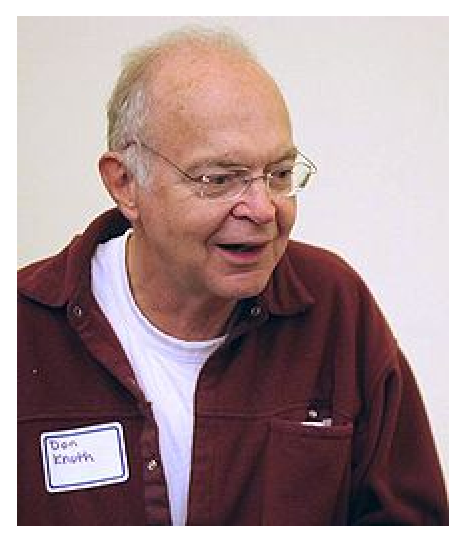
\includegraphics[width=0.25\linewidth]{knuth1}}
        \hfill
    }
    \caption{Подпись к картинке.}\label{fig:latex}
\end{figure}

Формулы в строку без номера добавляются так:
\[
    \lambda_{T_s} = K_x\frac{d{x}}{d{T_s}}, \qquad
    \lambda_{q_s} = K_x\frac{d{x}}{d{q_s}},
\]

Во \underline{\textbf{второй главе}} рассматривается метод вариации критической энергии в «резонансных» магнитооптиках. Для этого вводится суперпериодическая модуляция градиентов квадрупольных линз, тем самым варьируя дисперсионную функцию. Рассмотрен вопрос подавления хроматичности, а также нелинейных эффектов в таких структурах.

\underline{\textbf{Третья глава}} посвящена исследованию возможности прохождения критической энергии, характерней для регулярных структур. Исследована процедура скачка критической энергии. Данные численного моделирования, также апробированы на экспериментальной установке. 

Можно сослаться на свои работы в автореферате. Для этого в файле
\verb!Synopsis/setup.tex! необходимо присвоить положительное значение
счётчику \verb!\setcounter{usefootcite}{1}!. В таком случае ссылки на
работы других авторов будут подстрочными.
Изложенные в третьей главе результаты опубликованы в~\cite{vakbib1, vakbib2}.
Использование подстрочных ссылок внутри таблиц может вызывать проблемы.

В \underline{\textbf{четвертой главе}} рассматривается возможность исследования в комплексе Nuclotron–NICA электрического дипольного момента легких ядер. Для коллайдера NICA приведена возможность введения альтернативных каналов bypass. Рассматривается возможность модернизации Nuclotron.

\FloatBarrier
\pdfbookmark{Заключение}{conclusion}                                  % Закладка pdf
В \underline{\textbf{заключении}} приведены основные результаты работы, которые заключаются в следующем:
%% Согласно ГОСТ Р 7.0.11-2011:
%% 5.3.3 В заключении диссертации излагают итоги выполненного исследования, рекомендации, перспективы дальнейшей разработки темы.
%% 9.2.3 В заключении автореферата диссертации излагают итоги данного исследования, рекомендации и перспективы дальнейшей разработки темы.
\begin{enumerate}
  \item На основе анализа внутрипучкового рассеяния, а также стохастического охлаждения показано, что использование метода 'резонансной' структуры способно увеличить эффективность стохастического охлаждения. Особенно эффективным может быть использование 'комбинированной' структуры. Однако, эффекты ВПР для приведенных структуры оказались в несколько раз большими и в конечном счёте недостаточными, делая предпочтительной 'регулярную' структуру для тяжелоионного эксперимента.
  \item Для коллайдерных экспериментов с протонами рассмотрена 'резонансная' структура в варьированой критическая энергия, что использовано для рассмотрения адаптированной структуры коллайдера NICA.
  \item Численные исследования показали, что прохождение критической энергии может вызывать нестабильность продольного фазового движения. Использование процедуры скачка критической энергии может быть использовано для преодоления этой проблемы. Получены экспериментальные данные процедуры скачка критической с синхротрона У-70, которые находятся в соответствии с проведенным численными оценками с учетом высших порядков разложения коэффициента уплотнения орбиты и импедансов для различных интенсивностей сгустка.
  \item Использование процедуры скачка для коллайдера NICA ограничено величиной скачка критической энергии, а также для гармонического ВЧ темпом изменения критической энергии по сравнению с темпом ускорения пучка. Что делает невозможным использование процедуры для этого типа ВЧ. Для барьерного ВЧ приведены оценки продольной микроволновой неустойчивости, показывающие существенное ограничение на параметры конечного сгустка.
  \item Для исследования спиновой динамики и реализации "квази-замороженного" спина в коллайдере NICA рассмотрено введение обводных каналов bypass. На прямых участках предлагается расположение фильтров Вина для компенсации поворота спина под действием МДМ в магнитной арке.
  \item Рассмотрена модернизированная структура синхротрона Nuclotron с сохранением функции бустера поляризованного пучка в коллайдер NICA. В предложенных 8/16-периодичных структурах возможно проведение независимых прецезионных экспериментов по исследованию ЭДМ дейтрона и протона, а также осуществлению поика аксиона в режиме сканирующей антенны.
\end{enumerate}


\pdfbookmark{Литература}{bibliography}                                % Закладка pdf
При использовании пакета \verb!biblatex! список публикаций автора по теме
диссертации формируется в разделе <<\publications>>\ файла
\verb!common/characteristic.tex!  при помощи команды \verb!\nocite!

\ifdefmacro{\microtypesetup}{\microtypesetup{protrusion=false}}{} % не рекомендуется применять пакет микротипографики к автоматически генерируемому списку литературы
\urlstyle{rm}                               % ссылки URL обычным шрифтом
\ifnumequal{\value{bibliosel}}{0}{% Встроенная реализация с загрузкой файла через движок bibtex8
    \renewcommand{\bibname}{\large \bibtitleauthor}
    \nocite{*}
    \insertbiblioauthor           % Подключаем Bib-базы
    %\insertbiblioexternal   % !!! bibtex не умеет работать с несколькими библиографиями !!!
}{% Реализация пакетом biblatex через движок biber
    % Цитирования.
    %  * Порядок перечисления определяет порядок в библиографии (только внутри подраздела, если `\insertbiblioauthorgrouped`).
    %  * Если не соблюдать порядок "как для \printbibliography", нумерация в `\insertbiblioauthor` будет кривой.
    %  * Если цитировать каждый источник отдельной командой --- найти некоторые ошибки будет проще.
    %
    %% authorvak
    \nocite{vakbib1}%
    \nocite{vakbib2}%
    %
    %% authorwos
    \nocite{wosbib1}%
    %
    %% authorscopus
    \nocite{scbib1}%
    %
    %% authorpathent
    \nocite{patbib1}%
    %
    %% authorprogram
    \nocite{progbib1}%
    %
    %% authorconf
    \nocite{confbib1}%
    \nocite{confbib2}%
    %
    %% authorother
    \nocite{bib1}%
    \nocite{bib2}%

    \ifnumgreater{\value{usefootcite}}{0}{
        \begin{refcontext}[labelprefix={}]
            \ifnum \value{bibgrouped}>0
                \insertbiblioauthorgrouped    % Вывод всех работ автора, сгруппированных по источникам
            \else
                \insertbiblioauthor      % Вывод всех работ автора
            \fi
        \end{refcontext}
    }{
        \ifnum \totvalue{citeexternal}>0
            \begin{refcontext}[labelprefix=A]
                \ifnum \value{bibgrouped}>0
                    \insertbiblioauthorgrouped    % Вывод всех работ автора, сгруппированных по источникам
                \else
                    \insertbiblioauthor      % Вывод всех работ автора
                \fi
            \end{refcontext}
        \else
            \ifnum \value{bibgrouped}>0
                \insertbiblioauthorgrouped    % Вывод всех работ автора, сгруппированных по источникам
            \else
                \insertbiblioauthor      % Вывод всех работ автора
            \fi
        \fi
        %  \insertbiblioauthorimportant  % Вывод наиболее значимых работ автора (определяется в файле characteristic во второй section)
        \begin{refcontext}[labelprefix={}]
            \insertbiblioexternal            % Вывод списка литературы, на которую ссылались в тексте автореферата
        \end{refcontext}
        % Невидимый библиографический список для подсчёта количества внешних публикаций
        % Используется, чтобы убрать приставку "А" у работ автора, если в автореферате нет
        % цитирований внешних источников.
        \printbibliography[heading=nobibheading, section=0, env=countexternal, keyword=biblioexternal, resetnumbers=true]%
    }
}
\ifdefmacro{\microtypesetup}{\microtypesetup{protrusion=true}}{}
\urlstyle{tt}                               % возвращаем установки шрифта ссылок URL
